\section{Čistící filtr}

Byli navrženy 2 sady 4 filtrů typu pásmová zádrž na zablokování rušivých frekvencí (1 pro každou frekvenci).
Z grafů lze vidět, že Butterworthův filtr se po jednotkovém skoku nejrychleji ustálí na 0, ale aplituda zákmitů po před ustálením je vyšší než u Elliptic filtru.

\begin{figure}[H] 
	\centering
	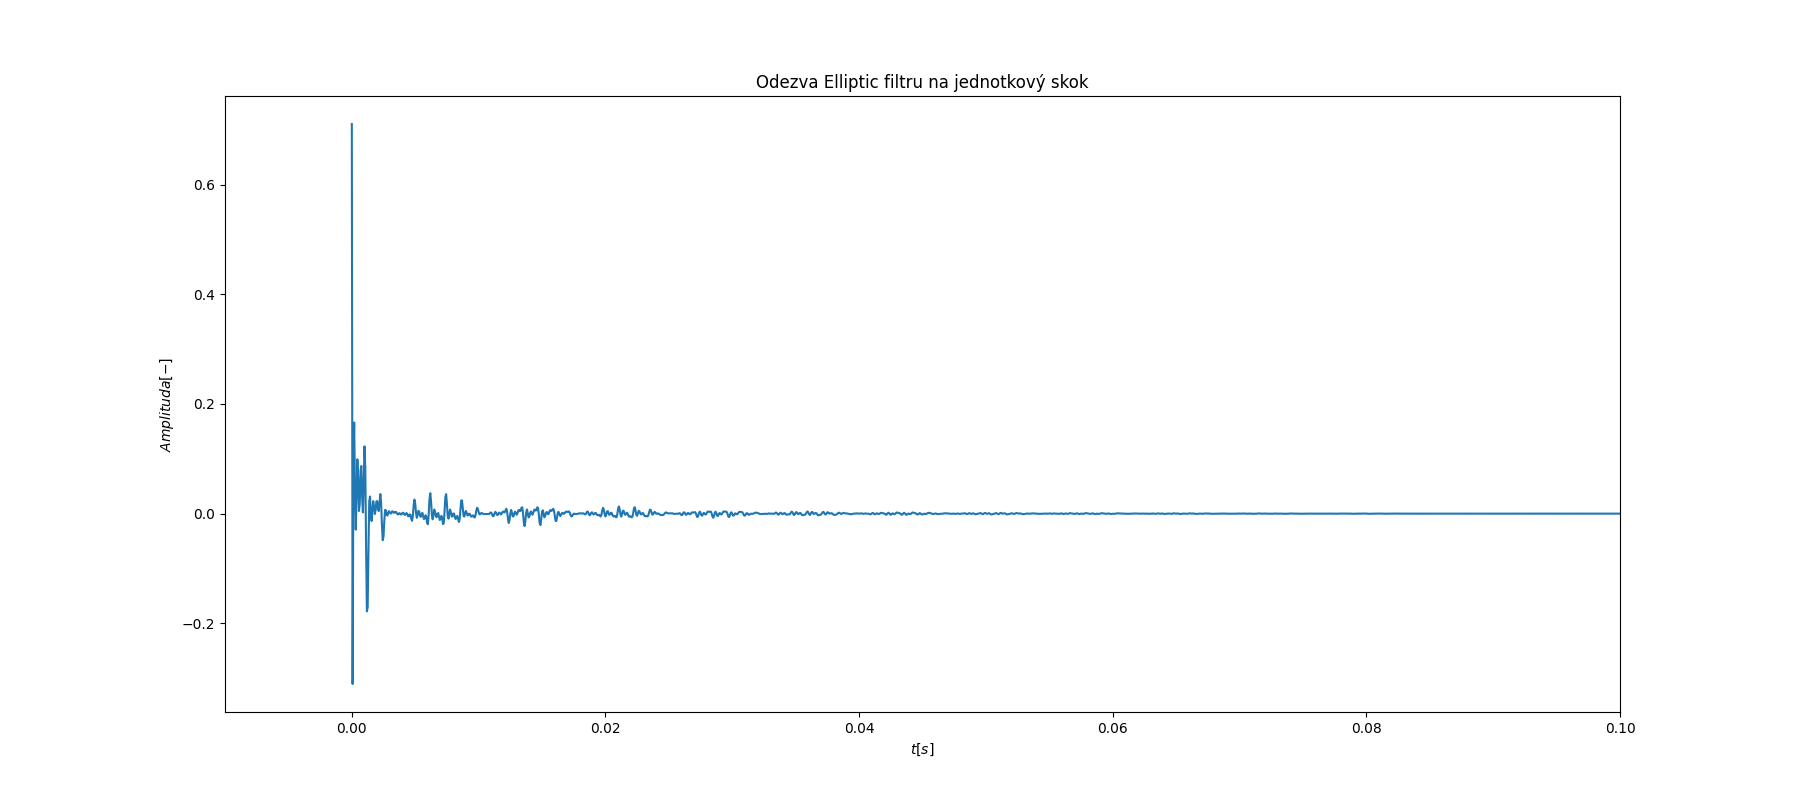
\includegraphics[scale=0.40,keepaspectratio]{Figure_22}
	\caption{Odezva na jednotkový skok Elliptic filtru}
\end{figure}

\begin{figure}[H] 
	\centering
	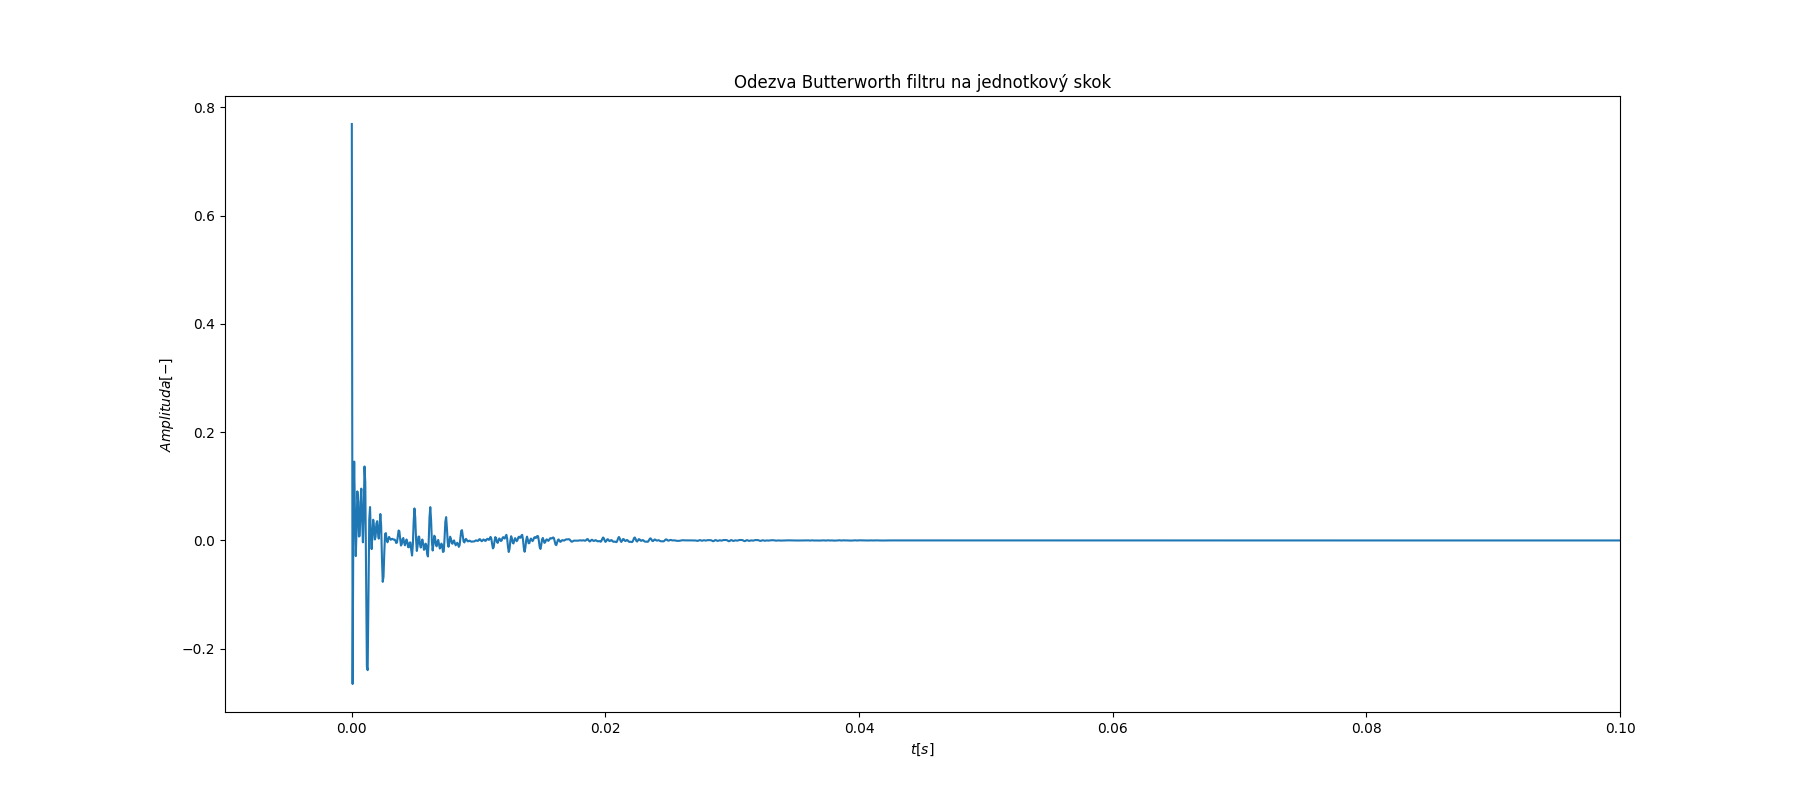
\includegraphics[scale=0.40,keepaspectratio]{Figure_24}
	\caption{Odezva na jednotkový skok Butterworth filtru}
\end{figure}